본 장에서는 이번 프로젝트의 타겟 게임인 슈퍼 마리오 브라더스 게임을 하위 섹션~\ref{sec:method:smb}에서 소개한다.

\subsection{슈퍼 마리오 브라더스}
\label{sec:method:smb}

\begin{figure}[h]
\begin{center}
\begin{tabular}{c}
     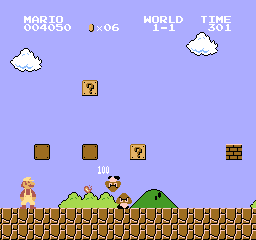
\includegraphics[width=0.45\textwidth]{FIG/SuperMarioBros.png} \\
\end{tabular}
\caption{
	슈퍼 마리오 브라더스의 게임 화면.
}
\label{fig:mario_title}
\end{center}
\end{figure}

슈퍼 마리오 브라더스는 닌텐도 초기의 액션 게임으로 1985년 9월 13일 NES (Nintendo Entertainment System) 전용 게임으로 출시 되었다.
Figure~\ref{fig:mario_title}은 이 게임의 플레이 화면이다.
당시 출시된 다른 게임들과 비교하여 우수한 조작감과 완성도 높은 미술로 크게 흥행하였으며 현재 2019년도 까지고 지속적으로 후속작이 출시되고 있다.
간단한 조작으로도 자유도 높은 플레이가 가능하여 강화학습의 목표로 삼기에 적합하여 이번 프로젝트의 대상으로 선택하였다.
슈퍼 마리오 브라더스는 총 8개의 world 와 각 world 당 4개의 stage로 구성되어 있다.
각 world 별로 특징있는 컨셉을 (물의 나라, 얼음의 나라, 등) 가지고 디자인 되어 배경 및 등장하는 적 케릭터가 차이가 있다.
또한 world 및 stage 수가 증가할 수록 난이도가 올라가는 경향을 가진다.

\begin{table}[h]
\centering
	\caption {
		슈퍼 마리오 브라더스에서 가능한 키 입력. 서로 다른 키를 조합하여 입력하는 것이 가능하다.
	}
	\label{tab:mario:key}
\begin{tabular}{ll}
\toprule
키     & \multicolumn{1}{c}{동작 설명} \\
\midrule
up    & 특수한 상황(넝쿨, 파이프)에서 마리오를 위로 이동 \\
left  & 마리오를 왼쪽으로 이동 \\
down  & 특수한 상황(넝쿨, 파이프)에서 마리오를 아래로 이동 \\
right & 마리오를 오른쪽으로 이동 \\
A     & 가속 또는 불꽃 공격(슈퍼 마리오만 해당)\\
B     & 점프 \\
\bottomrule
\end{tabular}
\end{table}

Table~\ref{tab:mario:key} 에서 슈퍼 마리오 브라더스 게임에서 가능한 모든 키 입력을 소개한다.
모든 입력은 중복하여 입력하여 마리오가 다른 동작을 하게 할 수 있다.
예를 들면 right 키와 B 키를 동시에 입력하면 마리오가 오른쪽으로 나아가며 점프한다.
하지만 경우에 따라 right 키와 left 키를 동시에 누른 경우 처럼 상보적인 두 가지 키를 조합하는 경우 무의미한 동작을 나타낼 수도 있다.
슈퍼 마리오 브라더스 게임에서 유의미한 키조합을 고려할 경우 가능한 Action의 경우의 수는 16가지 이다.

슈퍼 마리오 브라더스에서 목적지인 깃발로 이동하면 한 stage가 종료된다.
그 외에는 적에게 부딧치거나, 함정에 빠진 경우, 그리고 제한 시간이 지난 경우 stage가 종료되며 처음부터 다시 시작하게 된다.
이 게임의 목적은 보다 많은 점수를 얻으면서 깃발에 도달하여 stage를 완료하는 것이다.
stage 내부에서 점수를 얻는 방법은 아래와 같다.
\begin{itemize}
	\item \textbf{깃발 도달시 남은 시간:}
		제한 시간 이내에 깃발에 도달한 경우 남은 시간 (초 단위)당 100점 획득.
	\item \textbf{동전을 획득:}
		stage내에서 벽돌, 물음표 블록, 그리고 동전 아이템을 통해 동전에 닿으면 100점 획득.
	\item \textbf{버섯, 꽃을 획득:}
		stage내의 물음표 블록에서 버섯 또는 꽃이 나왔을 때 닿으면 100점 획득.
	\item \textbf{적을 처치:}
		적을 처치시 기본적으로 100점 획득하며 연속된 처치를 할 경우 매번 2배의 추가 점수 획득.
\end{itemize}

이 게임에서 stage별로 목적지에 도달하지 못하고 종료된 경우 다시 도전할 기회를 부여하는 데 이 횟수는 마리오의 남은 생명으로 결정된다.
게임내에서 녹색 버섯을 획득하거나 동전을 100개 모은 경우 추가로 보너스 생명을 1개 얻게 된다.
강화학습을 위한 환경에서는 학습을 시키기 위해 stage를 수 많이 반복하여야 하여 이러한 재도전 횟수를 제한하는 것을 해제한 상태에서 학습시키게 된다.
하지만 실제 플레이어가 게임을 한다고 가정할 때 이러한 생명을 관리하는 것은 게임을 끝까지 완수하기 위한 중요한 요소이다.
